\chapter{Testing}


This chapter will explore how testing has been accomplished in this research project, both day-to-day software testing, but also feedback from stakeholders and formal user testing. Because of the current COVID-19 pandemic, physical meeting and user testing been done sparingly, and have at times been impossible carry out, in fact the fall semester did not see any physical testing by users not affiliated with the VRLab at NTNU Dragvoll. What follows are the approach and structure of testing, research results and feedback from the testing sessions will be expanded further in the \nameref{chap:results} chapter.

\section{Software testing}
During development, software testing has been done unstructured, mostly by way of regular deployment and on-device feature testing. This is admittedly not the most comprehensive testing system and can not guarantee intended behavior as systems are combined and restructured, in the same way as a test suit with \textit{unit testing} and \textit{integration testing} could. But it allows for more rapid development, less overhead for a single developer and can not be said to have meaningfully limited the research project. A case could be made for a testing suit being helpful in the continuation of the research as new developers will have a concrete indication of intended behavior, this has and could not have a high priority as a development goal, because of limitations in development time and the demand for creating research results.

\section{Testing Precautions}

\subsection{Consent}
Every user tester where handed a consent form at the beginning of each session. This assured the privacy rights of the test persons, and gave approval to use the findings of the test session in this research. The consent form can be found in \autoref{appendix:consent}.

\subsection{Hygienic Measures}
Due to the COVID-19 pandemic, many new precautions have been enacted to prevent the spread of virtual pathogens. The most effective measure has undoubtedly been the limited number of testing sessions, even so what follow are the precautions taken during those physical meetings. 
Firstly, the general national guidelines of social distancing and clean hands were kept. 
Between each new person using a head mounted HoloLens 2, the headset was placed in a \textit{Cleanbox}, this is system specially design to disinfect AR and VR devices utilizing UVC radiation to destroy viruses. It claims to kill Covid-19 viruses with 99.999+\% efficacy\footnote{https://cleanboxtech.com}. Further, contact points and buttons on the device are swiped with alcohol-based sanitizer. The reason this step was not enough and the UVC box was needed is because of the fragile nature of the lenses of the AR device, it is generally recommended not to touch the lenses, and alcohol would naturally not be good. On Android devices this was however the main disinfection method as cellphones could be completely wiped. Lastly, the user would ware a hygienic mask under the headset which reduced contact between the user and the headset.
All in all these actions in combination with strict adherence to the national guidelines of physical distancing, washing and sanitizing of hands and waring of face masks were done to prevent spread of the virus. 

% zorro masks, UVC radiation, anti bacterial desinfactant, munnbind og avstand

\section{Stakeholder meetings}
Throughout the project, there have been multiple meetings with stakeholders from the Kavli Institute at St.Olavs. These have been a combination of physical meetings and virtual video conferences using Zoom. When meeting virtually the research prepared one or more video demonstrations captured on-device, either HoloLens 2 or Android, which were uploaded to YouTube for convenience. When meeting physically either the researcher or the stakeholder would use the application with live view enabled such that the other could see and comment on the usage. Afterwards, the progress was discussed and evaluated and feedback was given on usability and features. Primarily, the resulting feedback was in the form of feature request, and general technical in nature.
% Because of differing backgrounds the researcher and stakeholders had some communication issues,

\section{User Testing}
During the final stages of the research project, two user testing sessions were held. This both gave useful insight into what the application did well and badly. Many of the issues discovered in the first test session were improved upon, this process is explored in \autoref{chap:finaliter}. The last test session was at the end of the development phase on this project and was meant mainly to gather data for research. No further development has happened after this point and as such the last test session gives an accurate picture of the resulting software product of this research project, both in its proficiencies and its limitations. 

\begin{figure}[ht]
    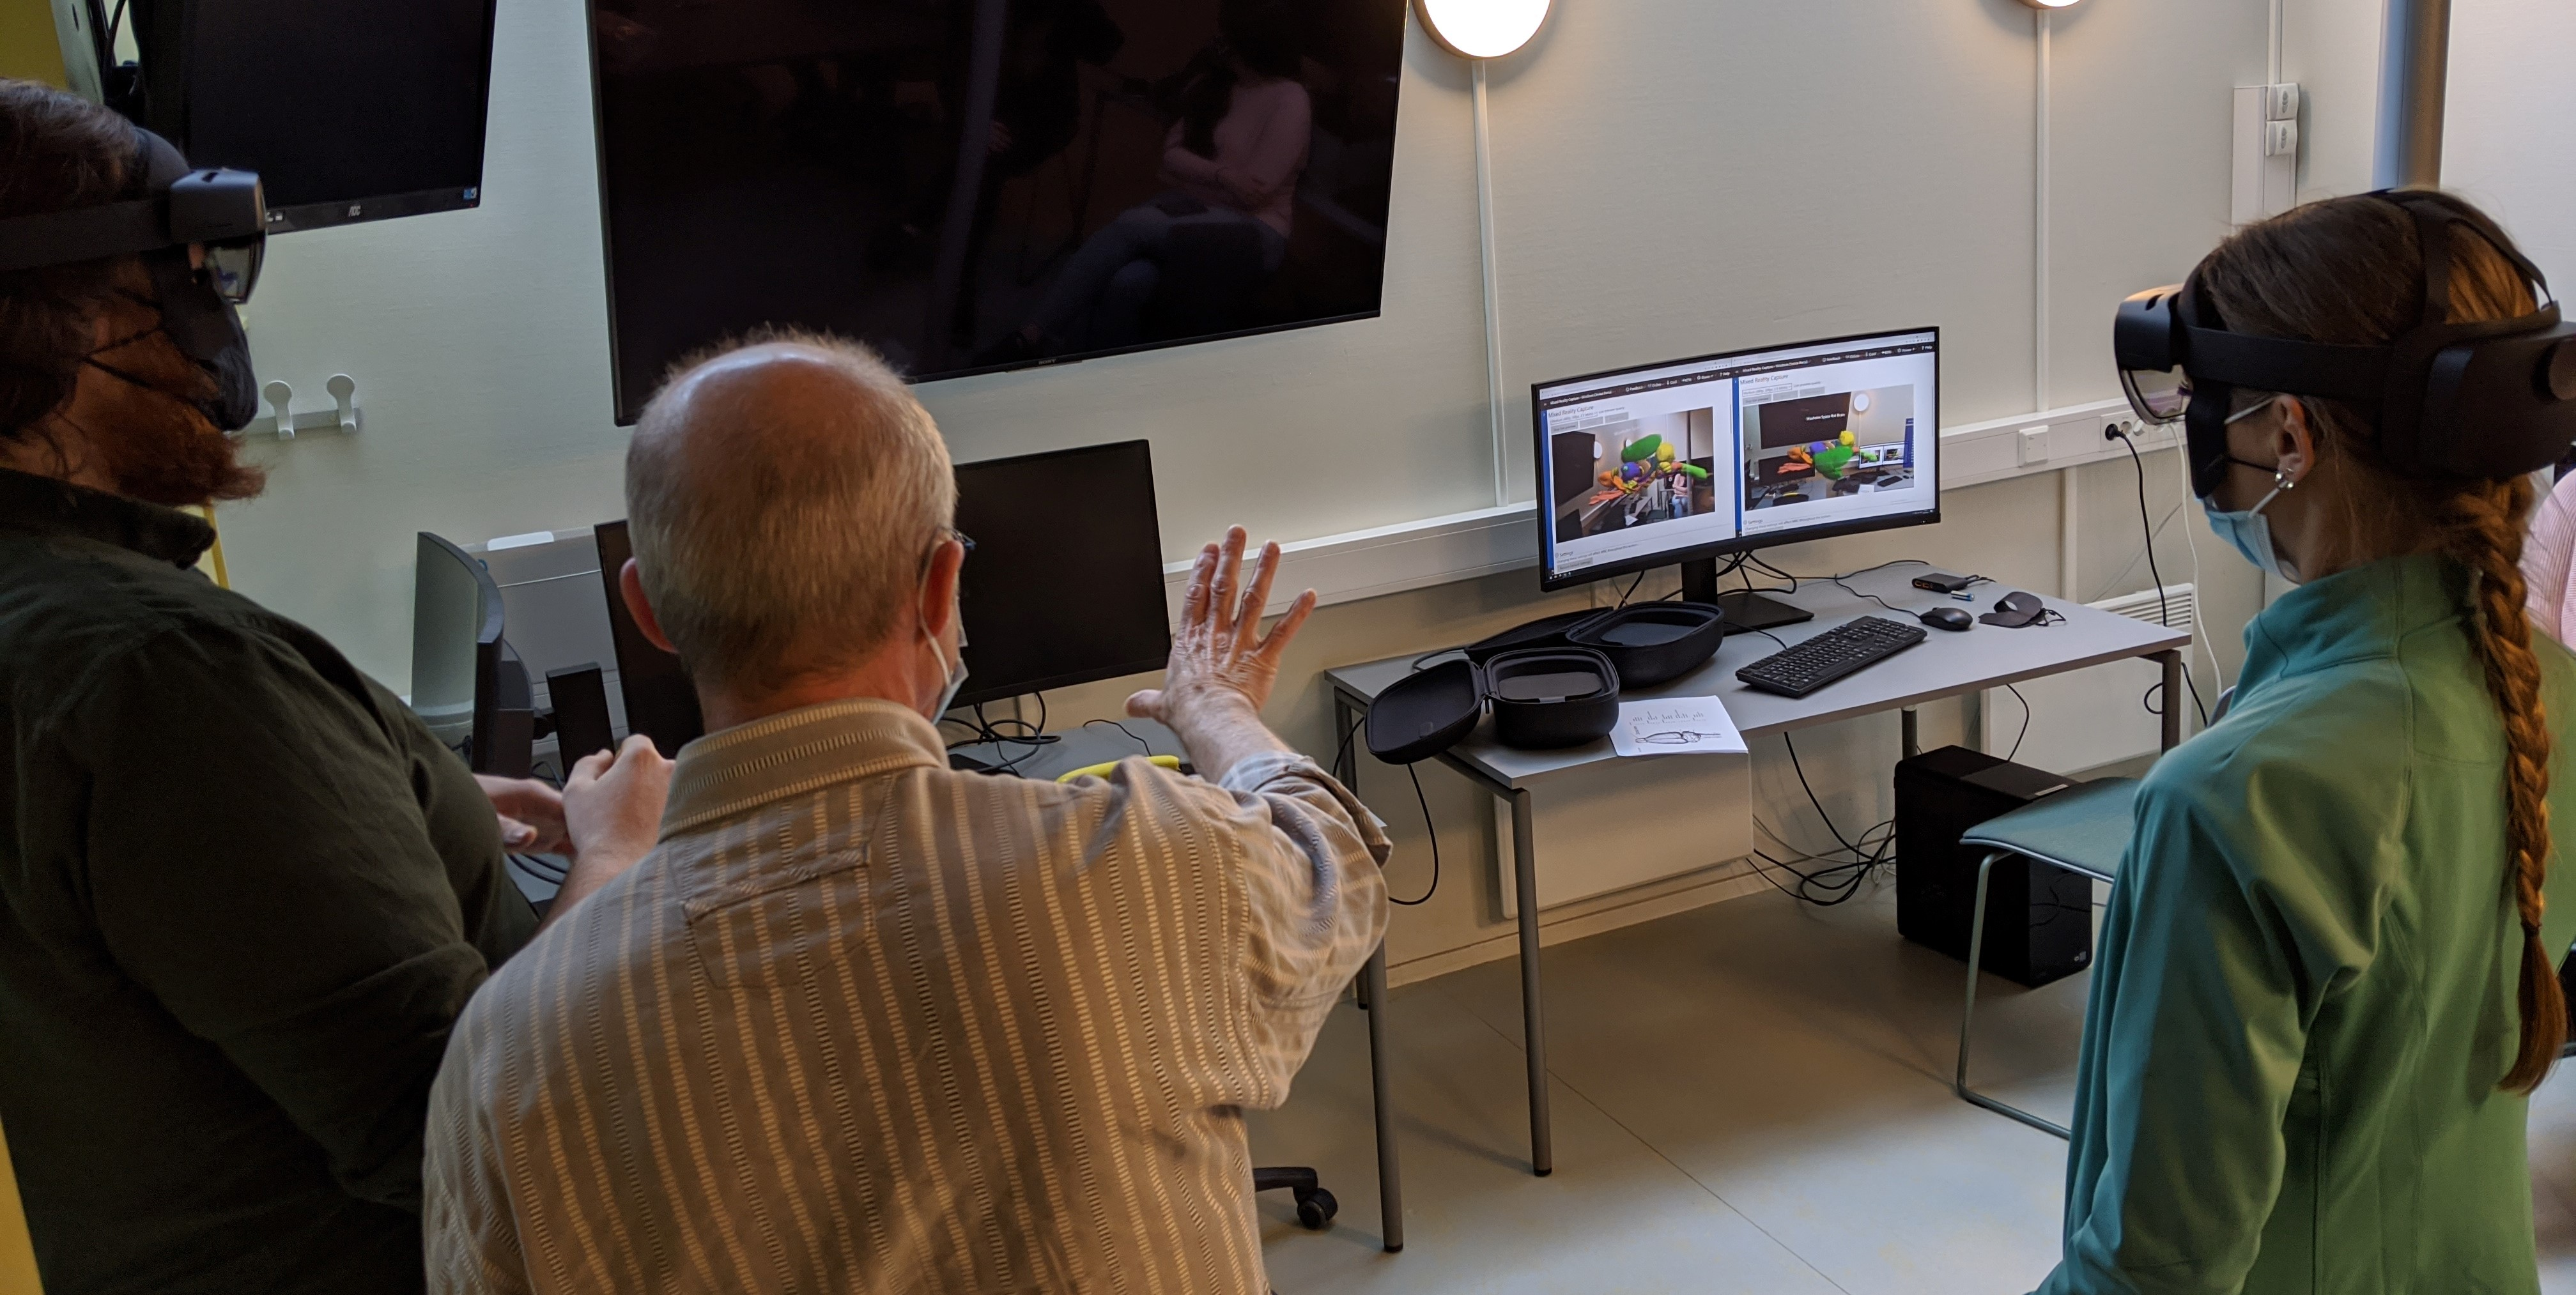
\includegraphics[width={\textwidth}]{fig/usertesthololivestream.jpg}
    \caption{Tester using HoloLens 2, being lectured by the neurologist whos watching their actions through live feed from Device Portal.}
    \label{fig:usertesthololivestream}
\end{figure}

\subsection{First testing session}

The first user testing had three participants, all being medical student. Two third year and one fifth year student. Additionally, one neurologist from the Kavli Institute was present in the role both of stakeholder in the research project and also as lecturer to the student whom all took courses held by the neurologist. This session did not test the Android application at all and only focused use with the HoloLens 2, this created a challenge for collaboration testing as only two HoloLens 2 devices were available. 

The session began by having the participants take a multiple choice test to survey their knowledge of the rat brain anatomy. This test was a standard test from course work in medical courses held by the stakeholder neurologist, and is meant to measure the short term learning from a single lecture. Therefore the exact same test was taken after the end of the session when the participants had used the research application.

After taking this test the participants were freely testing the application somewhat unstructured, and familiarizing them self with the usage of AR devices which none of the participants were accustomed with. Throughout the usage a pattern naturally evolved such that the neurologist lectured students with headset on. This started when the neurologist and a single student both used the application through the headset, the neurologist guided the student and showed them the different brain structures and explained there purpose. The one on one nature of these lectures were broken up by having the lecturer view the live stream of two students through a Windows desktop computer, this happened mostly because of time constraints as it lent itself to both of the remaining students having the lecture rather than just one. 
Both situations were insightful as observations of practical use of the application, and were not designed, nor intended by the researcher. 


% As this one on one lecturer continued it became apparent 
% While the neurologist used the headset in the beginning, which resulted in a one to one lecture s
% and was somewhat unstructured in its execution. This resulted in 

\subsection{Second testing session}



\begin{figure}
    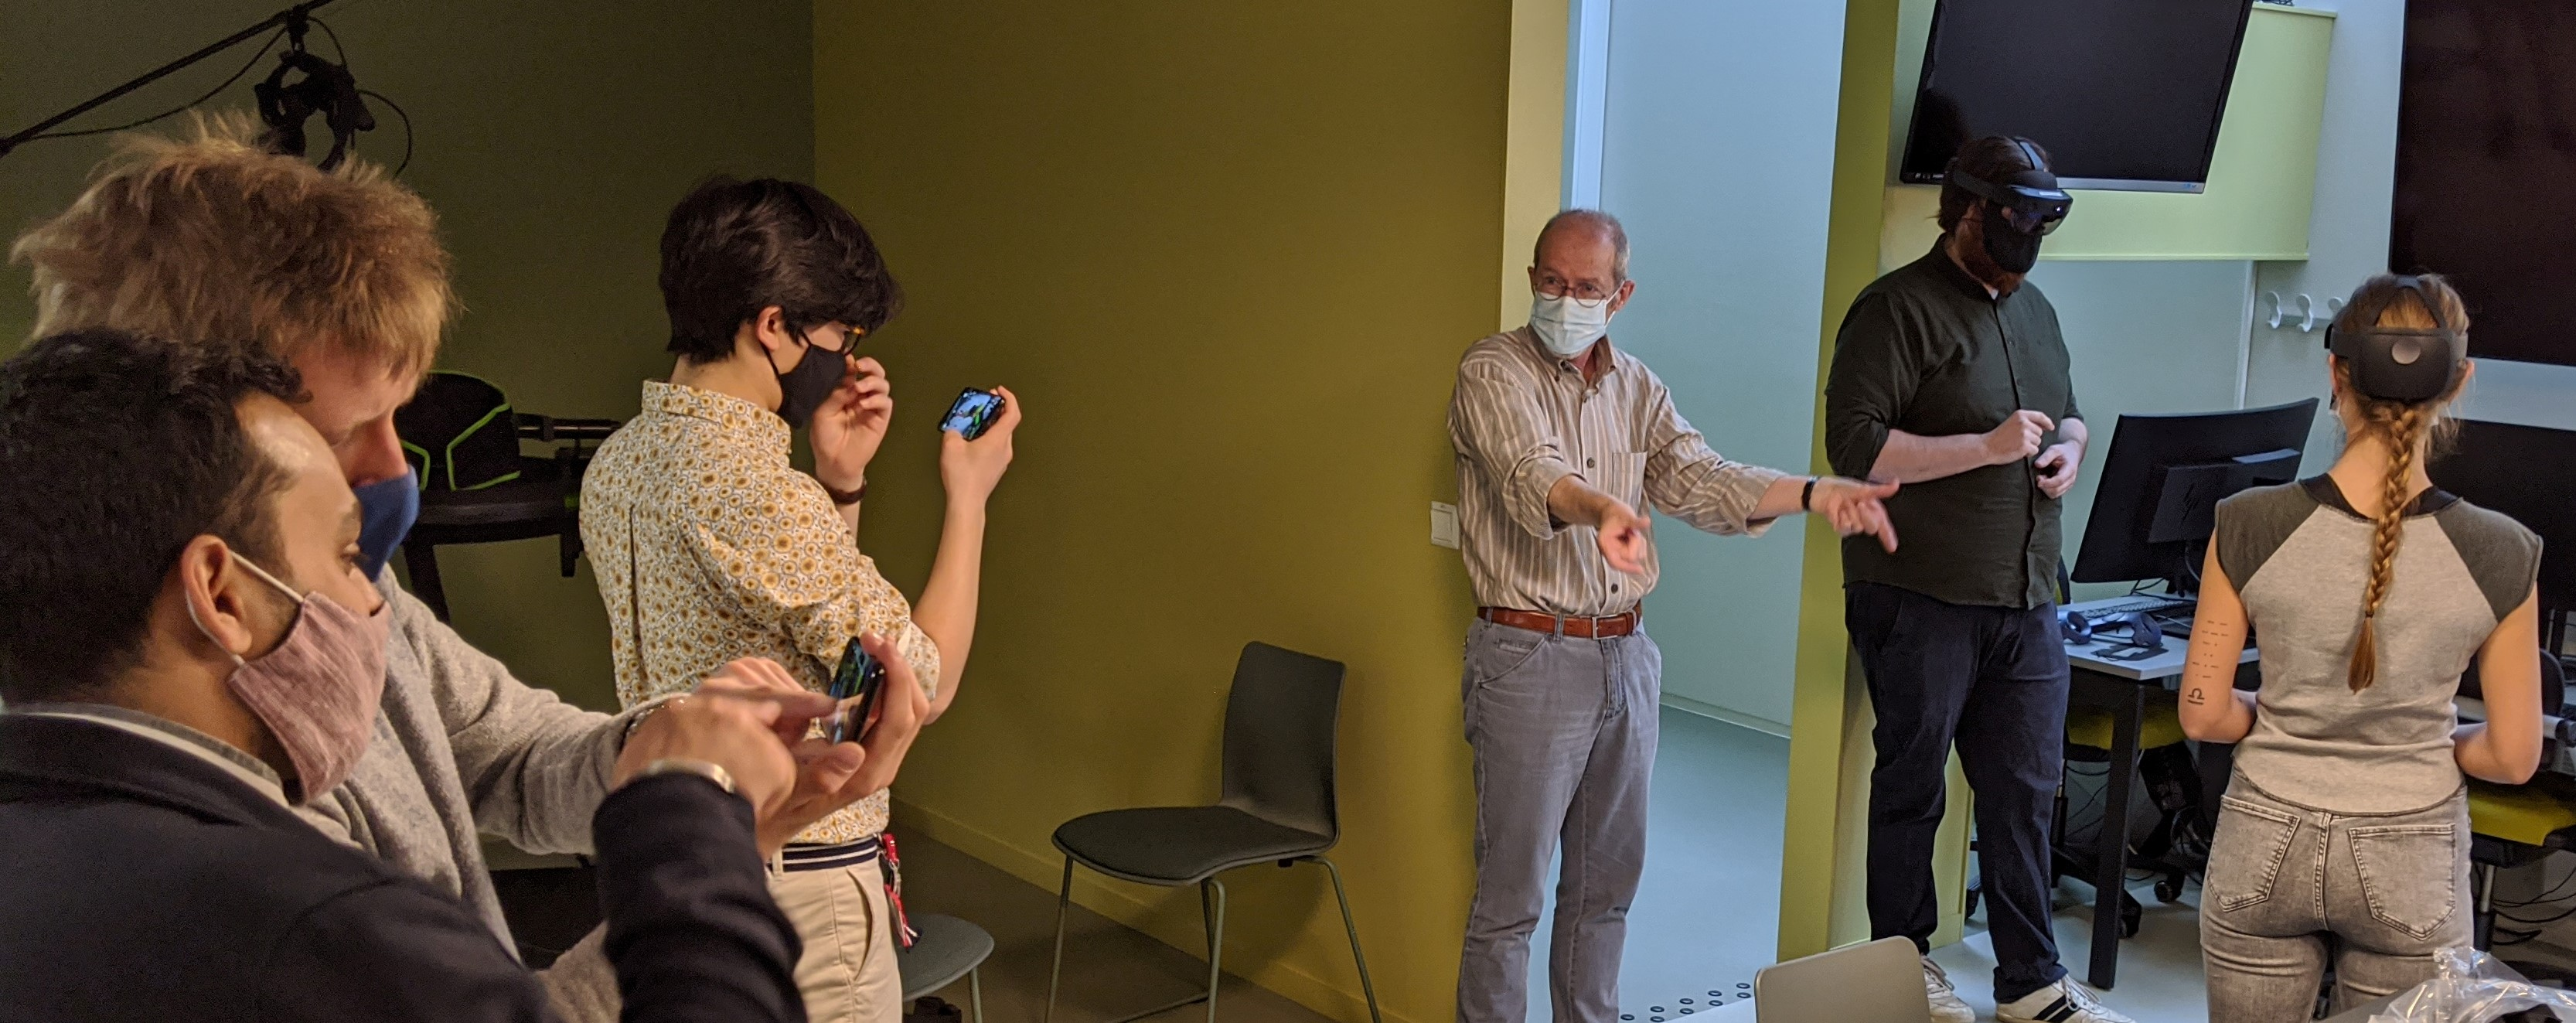
\includegraphics[width={\textwidth},trim={0 0 16cm 0},clip]{fig/usertestmennobeingmenno.jpg}
    \caption{Neurologist lecturing Android test users.}
    \label{fig:usertestmennobeingmenno}
\end{figure}


The second test session marked the end of this research projects development stage, thus it was a test of the final product in this research. Therefore, in addition to this test session being used for data gathering, it can also be seen as a final evaluation of the application. 

The participants in this session were five medical students, all first year and two computer science student. The session started as the previous one by having the participants filling out a consent from and taking the same initial knowledge test. 
The session was organized around the principle use case found in the previous test session where the neurologist lectured the participants, while himself seeing the application ran through live feed from the student participants.
This session tested with both HoloLens 2 as well as Android devices and thus two students could use the HoloLens 2 devices while another two could use Android smartphones. In \autoref{fig:usertestmennobeingmenno} the neurologist is explaining neuroanatomy to medical student who see the brain through both Android devices and HoloLens 2. The neurologist is seeing the view of the HoloLens 2 user through Windows Device Portal, which is not in the captured picture.
Afterwards, the participants took the same knowledge test and than a questionnaire. The questionnaire created by the researcher, was structure in three parts; a SUS questionnaire, general questions about use, thoughts and feedback to the application and last part was standardized questions used by NTNU VRLab about collaboration in XR. The questionnaire is attaches as \autoref{chap:questionnaire}.

\subsection{System usability scale}

System usability scale (SUS) is a questionnaire meant to measure a users subjective sense of a systems usability. It is built up of ten standardized questions which are general enough to apply to any user facing IT system. Questions are rated on a \textit{Likert scale}, meaning that each answer is a one to five rank ranging from strongly disagree to strongly agree. A complete SUS questionnaire can be found in the first section in the questionnaire used in this research at \autoref{chap:questionnaire}. By aggregating the results with a certain algorithm a score between 0 and 100 is generated. In the scoring system 68 is deemed a \textit{average} score and ranges from this and up to 80 is deemed \textit{good}, while above this is \textit{excellent}. Bellow this there is the {poor} rating down to 51 and even bellow that is called \textit{awful}.